%%%%%%%%%%%%%%%%%%%%%%%%%%%%%%%%%%%%%%%%%%%%%%%%%%%%%%%%%%%%%
%%%%%%%%%%%%%%%%%%%%%%%%%%%%%%%%%%%%%%%%%%%%%%%%%%%%%%%%%%%%%
%%
%%   NPR's ApJ template...  
%%   v1.0.0   Thu Dec  8 19:05:57 EST 2016
%%                                                                         
%%%%%%%%%%%%%%%%%%%%%%%%%%%%%%%%%%%%%%%%%%%%%%%%%%%%%%%%%%%%%
%%%%%%%%%%%%%%%%%%%%%%%%%%%%%%%%%%%%%%%%%%%%%%%%%%%%%%%%%%%%%
%\documentclass[manuscript]{aastex}
%\documentclass[twocolumn]{aastex61}
\documentclass{emulateapj}
%\documentclass[apj]{emulateapj}

\usepackage{graphicx,psfig,fancyhdr,natbib,subfigure}
\usepackage{epsfig, psfig, epsf}
\usepackage{amsmath, cancel}
\usepackage{amssymb}
%\usepackage{lscape}
\usepackage{dcolumn}% Align table columns on decimal point
\usepackage{bm}% bold math
\usepackage{hyperref,ifthen}
\usepackage{verbatim}



%%%%%%%%%%%%%%%%%%%%%%%%%%%%%%%%%%%%%%%%%%%
%       define Journal abbreviations      %
%%%%%%%%%%%%%%%%%%%%%%%%%%%%%%%%%%%%%%%%%%%
\def\nat{Nat} \def\apjl{ApJ~Lett.} \def\apj{ApJ}
\def\apjs{ApJS} \def\aj{AJ} \def\mnras{MNRAS}
\def\prd{Phys.~Rev.~D} \def\prl{Phys.~Rev.~Lett.}
\def\plb{Phys.~Lett.~B} \def\jhep{JHEP}
\def\npbps{NUC.~Phys.~B~Proc.~Suppl.} \def\prep{Phys.~Rep.}
\def\pasp{PASP} \def\aap{Astron.~\&~Astrophys.} \def\araa{ARA\&A}
\def\jcap{\ref@jnl{J. Cosmology Astropart. Phys.}} 
\def\nar{New~A.R.} 

\newcommand{\preep}[1]{{\tt #1} }

%%%%%%%%%%%%%%%%%%%%%%%%%%%%%%%%%%%%%%%%%%%%%%%%%%%%%
%              define symbols                       %
%%%%%%%%%%%%%%%%%%%%%%%%%%%%%%%%%%%%%%%%%%%%%%%%%%%%%
\def \Mpc {~{\rm Mpc} }
\def \Om {\Omega_0}
\def \Omb {\Omega_{\rm b}}
\def \Omcdm {\Omega_{\rm CDM}}
\def \Omlam {\Omega_{\Lambda}}
\def \Omm {\Omega_{\rm m}}
\def \ho {H_0}
\def \qo {q_0}
\def \lo {\lambda_0}
\def \kms {{\rm ~km~s}^{-1}}
\def \kmsmpc {{\rm ~km~s}^{-1}~{\rm Mpc}^{-1}}
\def \hmpc{~\;h^{-1}~{\rm Mpc}} 
\def \hkpc{\;h^{-1}{\rm kpc}} 
\def \hmpcb{h^{-1}{\rm Mpc}}
\def \dif {{\rm d}}
\def \mlim {m_{\rm l}}
\def \bj {b_{\rm J}}
\def \mb {M_{\rm b_{\rm J}}}
\def \mg {M_{\rm g}}
\def \mi {M_{\rm i}}
\def \qso {_{\rm QSO}}
\def \lrg {_{\rm LRG}}
\def \gal {_{\rm gal}}
\def \xibar {\bar{\xi}}
\def \xis{\xi(s)}
\def \xisp{\xi(\sigma, \pi)}
\def \Xisig{\Xi(\sigma)}
\def \xir{\xi(r)}
\def \max {_{\rm max}}
\def \gsim { \lower .75ex \hbox{$\sim$} \llap{\raise .27ex \hbox{$>$}} }
\def \lsim { \lower .75ex \hbox{$\sim$} \llap{\raise .27ex \hbox{$<$}} }
\def \deg {^{\circ}}
%\def \sqdeg {\rm deg^{-2}}
\def \deltac {\delta_{\rm c}}
\def \mmin {M_{\rm min}}
\def \mbh  {M_{\rm BH}}
\def \mdh  {M_{\rm DH}}
\def \msun {M_{\odot}}
\def \z {_{\rm z}}
\def \edd {_{\rm Edd}}
\def \lin {_{\rm lin}}
\def \nonlin {_{\rm non-lin}}
\def \wrms {\langle w_{\rm z}^2\rangle^{1/2}}
\def \dc {\delta_{\rm c}}
\def \wp {w_{p}(\sigma)}
\def \PwrSp {\mathcal{P}(k)}
\def \DelSq {$\Delta^{2}(k)$}
\def \WMAP {{\it WMAP \,}}
\def \cobe {{\it COBE }}
\def \COBE {{\it COBE \;}}
\def \HST  {{\it HST \,\,}}
\def \Spitzer  {{\it Spitzer \,}}
\def \ATLAS {VST-AA$\Omega$ {\it ATLAS} }
\def \BEST   {{\tt best} }
\def \TARGET {{\tt target} }
\def \TQSO   {{\tt TARGET\_QSO}}
\def \HIZ    {{\tt TARGET\_HIZ}}
\def \FIRST  {{\tt TARGET\_FIRST}}
\def \zc {z_{\rm c}}
\def \zcz {z_{\rm c,0}}


\newcommand{\sqdeg}{deg$^{-2}$}
\newcommand{\lya}{Ly$\alpha$\ }
%\newcommand{\lya}{Ly\,$\alpha$\ }
\newcommand{\lyaf}{Ly\,$\alpha$\ forest}
%\newcommand{\eg}{e.g.~}
%\newcommand{\etal}{et~al.~}
\newcommand{\cii}{C\,{\sc ii}\ }
\newcommand{\ciii}{C\,{\sc iii}]\ }
\newcommand{\civ}{C\,{\sc iv}\ }
\newcommand{\SiIV}{Si\,{\sc iv}\ }
\newcommand{\mgii}{Mg\,{\sc ii}\ }
\newcommand{\feii}{Fe\,{\sc ii}\ }
\newcommand{\feiii}{Fe\,{\sc iii}\ }
\newcommand{\caii}{Ca\,{\sc ii}\ }
\newcommand{\halpha}{H\,$\alpha$\ }
\newcommand{\hbeta}{H\,$\beta$\ }
\newcommand{\oi}{[O\,{\sc i}]\ }
\newcommand{\oii}{[O\,{\sc ii}]\ }
\newcommand{\oiii}{[O\,{\sc iii}]\ }
\newcommand{\heii}{[He\,{\sc ii}]\ }
\newcommand{\nii}{N\,{\sc ii}\ }
\newcommand{\nv}{N\,{\sc v}\ }

%% From:: /cos_pc19a_npr/LaTeX/proposals/JWST/JWST_ERS/Proposal/lines.tex
%%  
\newcommand{\imw}{$i$--$W3$}
\newcommand{\imwf}{$i$--$W4$}
\newcommand{\rmwf}{$r$--$W4$}
\newcommand{\imwt}{$i$--$W2$}
\newcommand{\wtmwf}{$W3$--$W4$}
%\newcommand{\kms}{km s$^{-1}$}
\newcommand{\cmN}{cm$^{-2}$}
\newcommand{\cmn}{cm$^{-3}$}
%\newcommand{\msun}{M$_{\odot}$}
\newcommand{\lsun}{L$_{\odot}$}
\newcommand{\lam}{$\lambda$}
\newcommand{\mum}{$\mu$m}
\newcommand{\ebv}{$E(B$$-$$V)$}
%\newcommand{\heii}{\mbox{He\,{\sc ii}}}
\newcommand{\cv}{\mbox{C\,{\sc v}}}
%\newcommand{\civ}{\mbox{C\,{\sc iv}}}
%\newcommand{\ciii}{\mbox{C\,{\sc iii}}}
%\newcommand{\cii}{\mbox{C\,{\sc ii}}}
%\newcommand{\nv}{\mbox{N\,{\sc v}}}
\newcommand{\niv}{\mbox{N\,{\sc iv}}}
\newcommand{\niii}{\mbox{N\,{\sc iii}}}
%\newcommand{\oi}{\mbox{O\,{\sc i}}}
%\newcommand{\oii}{\mbox{O\,{\sc ii}}}
%\newcommand{\oiii}{\mbox{[O\,{\sc iii}]}}
\newcommand{\oiv}{\mbox{O\,{\sc iv}}}
\newcommand{\ov}{\mbox{O\,{\sc v}}}
\newcommand{\ovi}{\mbox{O\,{\sc vi}}}
\newcommand{\ovii}{\mbox{O\,{\sc vii}}}

%\newcommand{\feii}{\mbox{Fe\,{\sc ii}}}
%\newcommand{\feiii}{\mbox{Fe\,{\sc iii}}}
%\newcommand{\mgii}{\mbox{Mg\,{\sc ii}}}
\newcommand{\neii}{[Ne\,{\sc ii}]\ }
\newcommand{\neiii}{[Ne\,{\sc ii}]\ }
\newcommand{\nev}{Ne\,{\sc v}\ }
\newcommand{\nevi}{[Ne\,{\sc vi}]\ }
\newcommand{\neviii}{\mbox{Ne\,{\sc viii}}}
\newcommand{\aliii}{\mbox{Al\,{\sc iii}}}
\newcommand{\siii}{\mbox{Si\,{\sc ii}}}
\newcommand{\siiii}{\mbox{Si\,{\sc iii}}}
\newcommand{\siiv}{\mbox{Si\,{\sc iv}}}
%\newcommand{\lya}{\mbox{Ly$\alpha$}}
%\newcommand{\lyb}{\mbox{Ly$\beta$}}
\newcommand{\hi}{\mbox{H\,{\sc i}}}
\newcommand{\snine}{\mbox{[S\,{\sc ix}]}}
\newcommand{\sivi}{\mbox{[Si\,{\sc vi}]}}
\newcommand{\sivii}{\mbox[{Si\,{\sc vii}]}}
\newcommand{\siix}{\mbox{[Si\,{\sc ix}]}}
\newcommand{\six}{\mbox{[Si\,{\sc x}]}}
\newcommand{\sixi}{\mbox{[Si\,{\sc xi}]}}
\newcommand{\caviii}{\mbox{[Ca\,{\sc viii}]}}
\newcommand{\arii}{\mbox{[Ar\,{\sc ii}]}}

%%[Ar II] 6.97
%% [S IX] 1.252 μm 328 
% [Si X] 1.430 μm 351 
% [Si XI] 1.932 μm 401 
% [Si VI] 1.962 μm 167 
% [Ca VIII] 2.321 μm 128 
% [Si VII] 2.483 μm 205 
% [Si IX] 3.935 μm 303
% [Ar II] 6.97


%\snine\ at 1.252$\mu$m, \six\ at 1.430$\mu$m, \sixi\ at 1.932$\mu$m, \sivi\ at
%1.962$\mu$m, \caviii\ at 2.321$\mu$m, \sivi\ at 2.483$\mu$m \siix\ at
%3.935$\mu$m and \arii\ at 6.97$\mu$m. 
%%
%% such as [Ne ii]12.8 μm, [Ne v]14.3 μm, [Ne iii]15.5 μm, [S iii]18.7 μm and 33.48 μm, [O iv]25.89 μm and [Si ii]34.8 μm (e.g
%%
%% MIR emission lines like [NeII] and [NeV] are ..
%%
%% Also,  arXiv:astro-ph/0003457v1 
%% [NeV] 14.32um & 24.32um and [NeVI] 7.65um imply an A(V)>160 towards the NLR...
%% [NeIII]15.56um/[NeII]12.81um
%%
%% [Ne V] 14.3, 24.2 μm 97.
%% [Ne II] 12.8 μm
%% [OIV] 26μm
%%


\begin{document}

\shorttitle{MIR Variable Quasars}
\shortauthors{N.~P.~Ross {\it et al.}}

\title{Mid-IR Variability of Quasars:  \\
       Typical Values and Extreme Outliers
}
\author{
Nicholas~P.~Ross\altaffilmark{1}, 
Aaron~ Meisner\altaffilmark{2}, 
Daniel~Stern\altaffilmark{3},
David~J.~Schlegel\altaffilmark{2},
Matthew~Graham\altaffilmark{4}, 
Arjun~Dey\altaffilmark{5},
Roberto~J.~Assef\altaffilmark{6},
Saavik~K.~Ford,\altaffilmark{7}, 
Barry~L.~McKernan\altaffilmark{7},
Mislav~Balokovic\altaffilmark{6}, 
Murray~Brightman\altaffilmark{4}, 
Andrew~Drake\altaffilmark{4}, 
Peter~R.~Eisenhardt\altaffilmark{3}, 
}
\altaffiltext{1}{Institute for Astronomy, University of Edinburgh, Royal Observatory, Blackford Hill, Edinburgh EH9 3HJ, United Kingdom}
\email{npross@roe.ac.uk}
\altaffiltext{2}{Lawrence Berkeley National Laboratory, 1 Cyclotron Road, Berkeley, CA 92420, U.S.A.} 
\altaffiltext{3}{Jet Propulsion Laboratory, California Institute of Technology, 4800 Oak Grove Drive, Mail Stop 169-221, Pasadena, CA 91109, USA}
\altaffiltext{4}{California Institute of Technology, 1200 East California Boulevard, Pasadena, CA 91125, USA}
\altaffiltext{5}{Steward Observatory, 933 North Cherry Avenue, Tucson, AZ 85721, U.S.A.}
\altaffiltext{6}{Universidad Diego Portales, Av Republica 180, Santiago, Regi ́on Metropolitana, Chile}
\altaffiltext{7}{Department of Astrophysics is located in the Rose Center for Earth and Space, American Museum of Natural History, Central Park West at 79th Street, New York, NY 10024, U.S.A}


\date{\today}

\begin{abstract}
In this paper we present the mid-infrared, light-curves for 248 quasars that show large, $>0.5$
mag peak-to-peak variation, in either the W1 or W2 (3.4 or 4.6 $\mu$m)
bands. Our motivation is to quantify and understand the ubiquity and
processes involved in luminous AGN obscuration.  The quasars are part
of the SDSS-I/II or SDSS-III: BOSS Quasar surveys, a superset of over
300,000 objects with at least one epoch of spectroscopy. The IR light
curves are from the WISE, NEOWISE and NEOWISE-R missions. 
%%
Critically we employ new DECaLS data, and find objects that were
`traditional' blue quasars (and appear so in SDSS imaging) but turn to
red in color in DECaLS, and are often extended.
%%
In particular, we present the $z=0.378$ quasar SDSS
J110057.70-005304.5 as a quasar that is tranistioning from a blue
continuum sloped object to become a ``Changing-Look'' quasar (with the
prominence of the H$\beta$ and H$\gamma$ broad-emission lines being
dramatically reduced. What makes J110057 particularly interesting,
however, is (by selection) its associated short-term IR variablity,
and dramatic reddening in the optical continuum during the transition
to its CLQ state.
%%
(TBD:: ) We explore simple models of quasar obscuration, and given the
short observed timescales ($\approx$7 years in the rest frame) find it
very hard to explain this behaviour.
\end{abstract}

\keywords{WISE, QSOs}

\maketitle


%%%%%%%%%%%%%%%%%%%%%%%%%%%%%%%%%%%%%%%%%%%%%%%%%%%%%%%%%%%%%
%%%%%%%%%%%%%%%%%%%%%%%%%%%%%%%%%%%%%%%%%%%%%%%%%%%%%%%%%%%%%
%%
%%   SECTION 1  SECTION 1  SECTION 1  SECTION 1  SECTION 1  SECTION 1  
%%   SECTION 1  SECTION 1  SECTION 1  SECTION 1  SECTION 1  SECTION 1  
%%   SECTION 1  SECTION 1  SECTION 1  SECTION 1  SECTION 1  SECTION 1  
%%
%%%%%%%%%%%%%%%%%%%%%%%%%%%%%%%%%%%%%%%%%%%%%%%%%%%%%%%%%%%%%
%%%%%%%%%%%%%%%%%%%%%%%%%%%%%%%%%%%%%%%%%%%%%%%%%%%%%%%%%%%%%
\section{Introduction}
The reprocessing of UV/optical photons by micron sized carbonates and
silicates around an AGN central engine leads to the prodigious emission
of infrared (IR) emission (\citet[See][for review on AGN infrared
emission]{Elitzur14}; \citet[][for a review on the Unified Model of
Active Galactic Nuclei]{Netzer15} and \citet[][]{Draine03} for a
review on dust).
%% All these References will need to be fixed/heavily updated.

With the energy released by the accretion of material onto a galactic
central engine black hole being comparable to the energy released in
nuclear fusion (REFs!!) having a full accounting of the bolometric
output from a luminous AGN, i.e. a quasar, is a critical part of any
contemporary galaxy and AGN model and evolutionary theory (e.g. current
Illustrious and EAGLE refs??). Thus, identifying AGN in the IR, and in
particular at $\sim$10$\mu$m where the AGN contribution to the SED
peaks (REFs) is of key interest. Indeed, many studies have explored
the utilization of mid-IR (3-30$mu$m rest) to identify and characterize
AGN and quasars \citep{Lacy04, Stern05, Martinez-Sansigre06,
Richards09b, Donley12, Stern12, Banerji13, Assef13, Richards15,
Timlin16}. 

Along with the raw energy output, of further critical importance to
understanding in detail the physical processes of the AGN, and the
potential for ``feedback'' on the host galaxy, is the time-dependent
nature of the obscuring, dusty material. Although this is thought to
be a dusty rotating ``torodial'' structure on $\sim$parsec scales,
apart from a few very local case studies (e.g. VLT MIR interferometry
objects) we are currently very ignorant to the geometry and topology
of the AGN IR emitting region.

As such, observing, and characterizing the MIR {\it light curves} (LCs) of
luminous AGN, would garnish major clues into the variable nature of
the energy output of the central engine, along with key tests and
constraints on the ``AGN unified model''.

In this paper{\it Letter}, we use the data from the Wide-Field
Infrared Survey Explorer \citep[WISE; ][]{Wright10}, and in particular
the NEOWISE-R mission \citep{Mainzer14, Meisner16}, combined with the
Sloan Digital Sky Survey quasar catalogs \citep[DR7Q][]{Schneider10}
and Dark Energy Camera Legacy Survey \citep[DECaLS][]{Lang16} to
identify 105 quasars (from a sample of 105,000) with large changes,
$|\Delta$ mag$|>0.5$, in their MIR LCs. This is the first time a
sample of quasars with varying MIR photometry has been observed. (IS
THIS TRUE??!?!!!)

In Section 2 we describe our datasets and methods for finding the MIR
variable quasars, including false positive checks. In Section 3 we
present our sample and the place the Extreme-IR Changers in context of
the general QSO population. In Section 4 we {\it potentially} say
``something'' about obscuration rates and draw our conclusions. 
The (online) Appendix gives the full details or our sample. 
%%
Because of established conventions, we report SDSS magnitudes on the
AB zero-point system \citep{Oke83, Fukugita96}, while the WISE
magnitudes are calibrated on the Vega system \citep{Wright10}.

%%%%%%%%%%%%%%%%%%%%%%%%%%%%%%%%%%%%%%%%%%%%%%%%%%%%%%%%%%%%%%
%%%%%%%%%%%%%%%%%%%%%%%%%%%%%%%%%%%%%%%%%%%%%%%%%%%%%%%%%%%%%%
%%
%%   S E C T I O  N   2         S E C T I O  N   2          S E C T I O  N   2        S E C T I O  N   2
%%   S E C T I O  N   2         S E C T I O  N   2          S E C T I O  N   2        S E C T I O  N   2
%%   S E C T I O  N   2         S E C T I O  N   2          S E C T I O  N   2        S E C T I O  N   2
%%
%%%%%%%%%%%%%%%%%%%%%%%%%%%%%%%%%%%%%%%%%%%%%%%%%%%%%%%%%%%%%%
%%%%%%%%%%%%%%%%%%%%%%%%%%%%%%%%%%%%%%%%%%%%%%%%%%%%%%%%%%%%%%
\section{Data}
We utilize three large datasets for our investigations: the 5-band,
optical Sloan Digital Sky Survey (SDSS; all the usual refs), the
3-band optical Dark Energy Camera Legacy Survey
\citep[DECaLS]{Lang16}, and data from the WISE mission. Crucially,
data from all three surveys is combined, details of which can be found
at \href{legacysurvey.org}{\tt legacysurvey.org}. We summarize the
salient details here.

\subsection{Optical Data}
    \subsubsection{SDSS and SDSS-III: BOSS}
    The SDSS is described in full detail elsewhere \citep{Fukugita96,
      Gunn98, York00, Hogg01, Lupton01, Stoughton02, Smith02, Pier03,
      Ivezic04, Gunn06, Tucker06, Padmanabhan08a}. The third incarnation of
    the SDSS, SDSS-III is described in \citet{Eisenstein11} with the
    Baryon Oscillation Spectroscopic Survey (BOSS) being detailed in
    \citet{Dawson13}. The final data release paper from SDSS-III was the
    Data Release 12 \citep{DR12}.
    
    We use the SDSS Seventh Data Release Quasar Catalog
    \citep[DR7Q;][]{Schneider10, Shen11} and the SDSS-III Twelve Data
    Release \citep[DR12Q;][]{Paris16}. SDSS quasar targets with
    $i\leq19.1$ were selected if the colors were consistent with being at
    redshift $z\lesssim3$, and $i\leq20.2$ objects were selected if
    $z\gtrsim$3, as outlined in \citet{Richards02}. BOSS quasar targets
    are selected to a magnitude limit of $g \leq 22.0$ or $r\leq 21.85$,
    with the primary goal to select quasars in the redshift range $2.2\leq
    z \leq 3.5$ as described by \citet[][and references
    therein]{Ross12}. In both SDSS and BOSS, quasar targets are also
    selected if they are matched within 2$''$ (1$''$ in the case of BOSS)
    of an object in the Faint Images of the Radio Sky at Twenty-cm (FIRST)
    catalog of radio sources \citep{Becker95}. Both the SDSS DR7Q and
    BOSS DR12Q include quasars that were selected by algorithms other than
    the main quasar selections; these sources appear in the catalog due
    to being targeted by the respective galaxy selections, being a
    `serendipitous' \citep{Stoughton02} or `special' \citep{DR4} target in
    SDSS, or an `ancillary' target in BOSS \citep[][]{Dawson13, DR12, DR14}.
    
    \subsubsection{SDSS and SDSS-III: BOSS}
    The Dark Energy Camera Legacy Survey \citep[DECaLS; ][]{Lang16} is
    taking deep 3-band $g,r,z$ imaging over 10,000deg of the Northern Sky
    that is accessible from the Cerro Tololo International Observatory
    site. As of writing the DECaLS is ongoing, with the latest data release being
    the Data Release 3 (DECaLS DR3). 
    
    
    \subsection{Infrared Data}
    As noted in \citet{Maizner14} and \citet{Meisner16}, after its
    initial launch, cryogenic mission, and a period of hibernation, the
    WISE satellite was reactivated, and recommenced surveying the sky in
    its two shorter wavebands, $W1$ and $W2$.  This W1/W2 survey is
    referred to as NEOWISE-Reactivation or NEOWISER.
    
    We directly use the data from \citet{Meisner16} which employs an
    adaptation of the unWISE \citet{Lang14} image coaddition framework.
    
    {\it From Aaron's email Oct 13, 2016}.
    http://legacysurvey.org/dr3/catalogs
    
    But if you look at the Tractor catalog column descriptions, you will
    see that DR3 includes sparse WISE W1/W2 light curves for every
    optically detected source (WISE\_LC*). These WISE light-curves are
    measured by forced-photometry of time-resolved unWISE coadds.
    Currently, in the DECaLS footprint, there are typically four epochs,
    sometimes five, and very rarely only three. These light curves
    typically span a $\sim$4-5 year time baseline, $\sim$2010-2014.

%% I created the time-resolved unWISE coadds that were the basis of these
%% light curves, so let me know if you have any further questions. I
%% would hope that the way they are packaged into the Tractor catalogs
%% will make them very straightforward to use. The most obvious
%% application of these light curves is indeed quasar variability,
%% whether for DESI targeting or quasar science in its own right.
%% Unfortunately I don't currently have time to do these science projects
%% myself, but I hope you will find these light curves useful and keep me
%%in the loop about your findings. Thanks.


\begin{figure}
  %% trim=l b r t 
  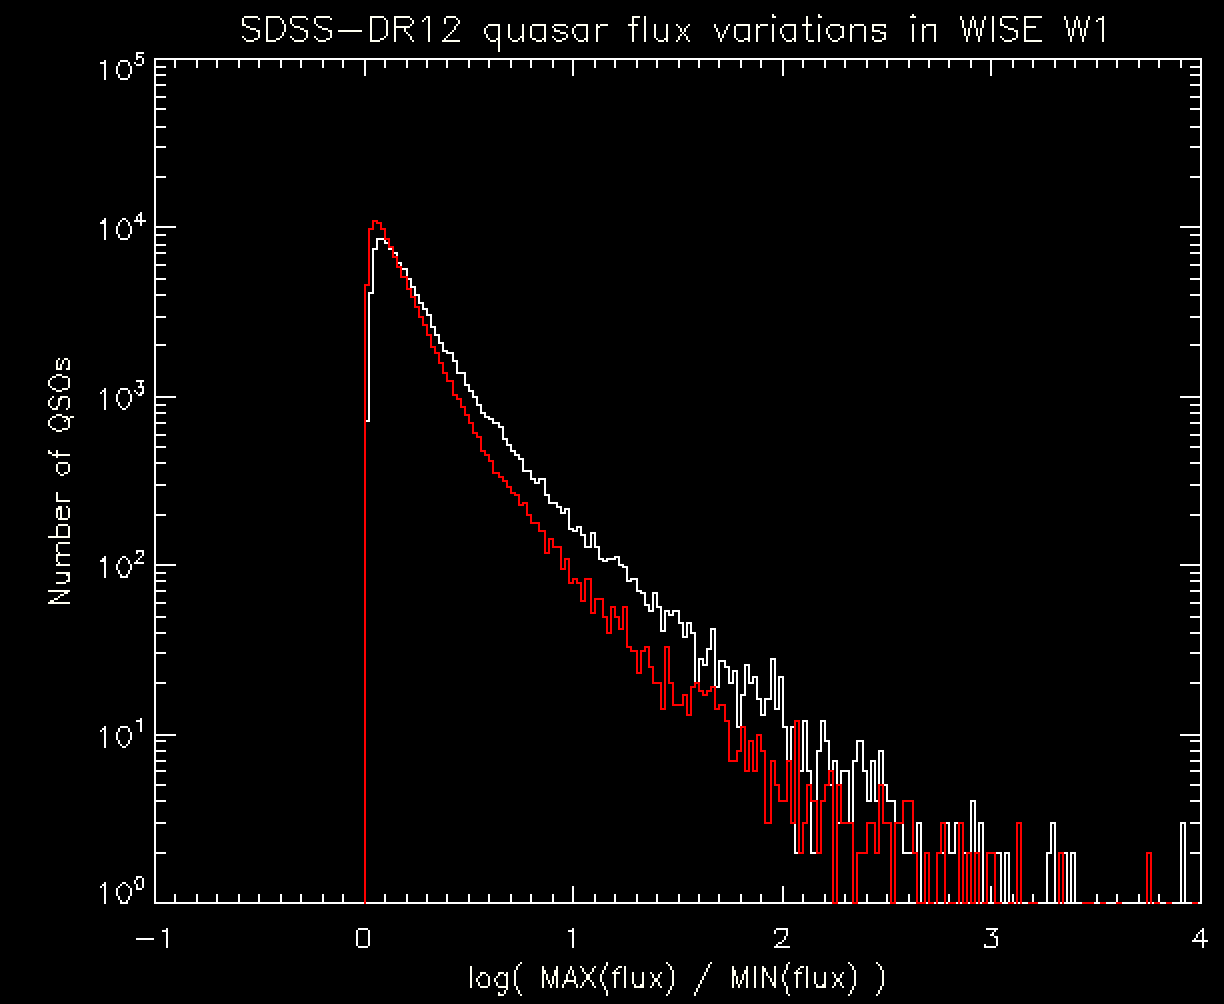
\includegraphics[width=8.00cm, height=7.50cm, trim=0.0cm 0.0cm 0.0cm 0.0cm, clip]
  {fig1.png}
  \centering
  % \vspace{-16pt}
  \caption[]{
    {\bf All from DJS's email:} The distribution of the maxima and
    minima flux in $W1$ for the $\sim$240k high-confidence quasars in the
    SDSS-III: BOSS DR12.  The red distribution is if one replaces fluxes
    with a mean flux$+$measurement error for each observation.  Note,
    since the log is being plotted, the difference between the two lines
    shows a significant variable population.  There are $\sim$1000 quasars
    where the $W1$ flux varies by more than a factor of 2 with a $>5$
    sigma confidence.  Some have a poor $\chi{^2}$ fits.
  }
 \label{fig:maxminflux}
\end{figure}
The distribution of the maxima and minima flux in $W1$ for the
$\sim$240k high-confidence quasars in the SDSS-III: BOSS DR12 is given
in Figure~\ref{fig:maxminflux}.

\begin{figure}
  %% trim=l b r t 
  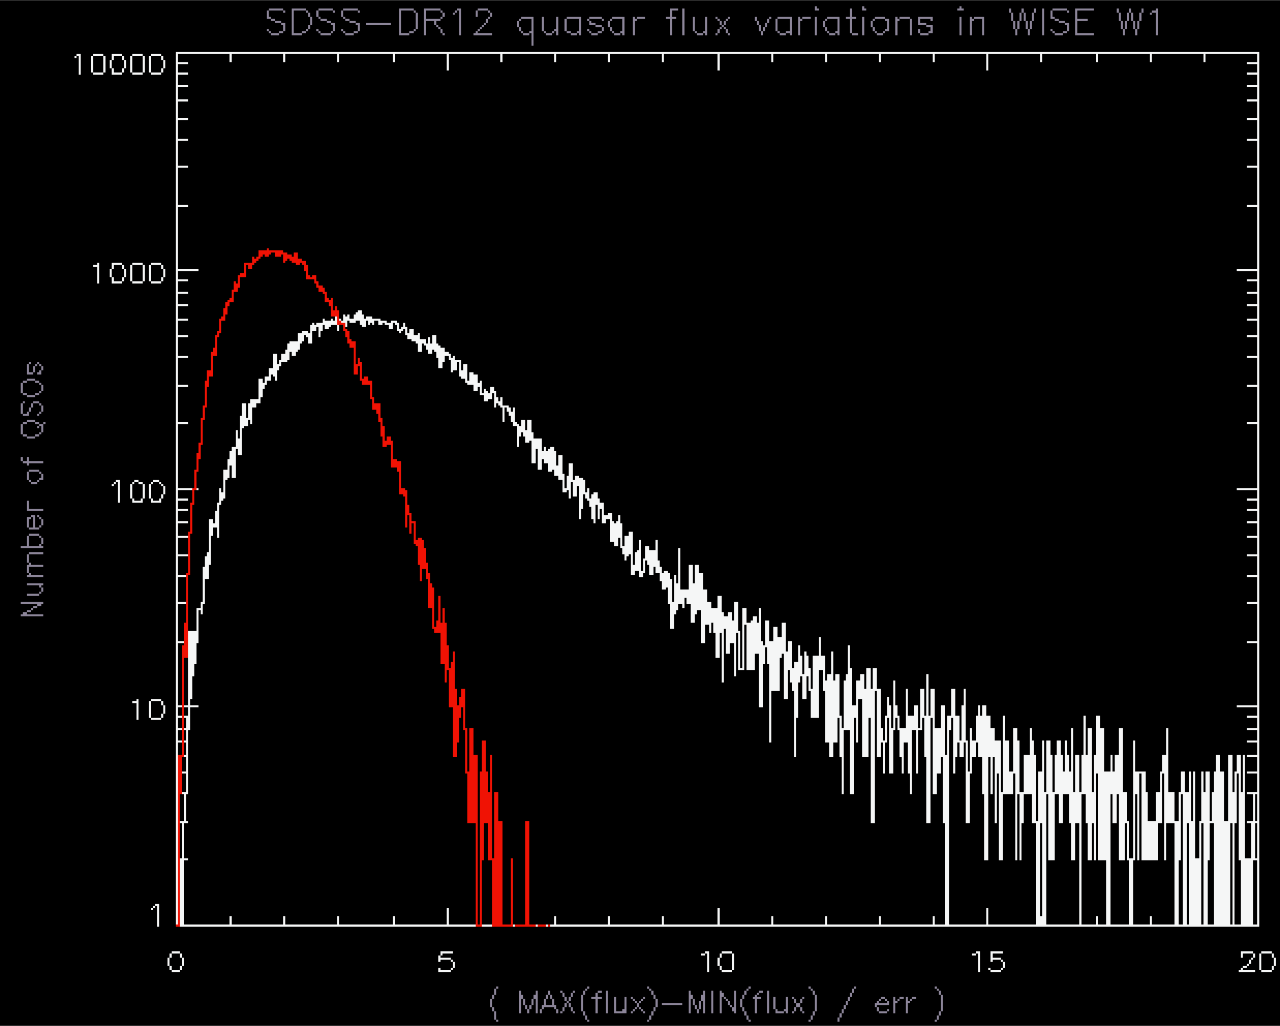
\includegraphics[width=8.00cm, height=7.50cm, trim=0.0cm 0.0cm 0.0cm 0.0cm, clip]
  {fig2.png}
  \centering
  % \vspace{-16pt}
  \caption[]{
    {\bf All from DJS's 2nd email:} 
Here, ``err'' is the quadrature sum of the errors at the minimum and maximum fluxes.
The red histogram is the expected distribution if these objects had no variability, 
and the errors were normally-distributed for each of the epochs.
This shows that $\sim6,000$ quasars are $>10\sigma$ detections of variability in W1.
%Though I still haven’t done this carefully enough to reject the poor chi^2 in individual WISE fits, etc.
  }
 \label{fig:maxmin_err}
\end{figure}
\subsection{``False Postive Checks''}
Figure~\ref{fig:maxmin_err} is the distribution of (max-min)/error in
the MIR fluxes.  (Should also be looking at the SDSS stars as a
control sample (don’t have those on my laptop).  The WISE magnitude
range for those stars will be quite different, though, since they have
the same optical magnitude range but are fainter in WISE.)



\begin{figure}
    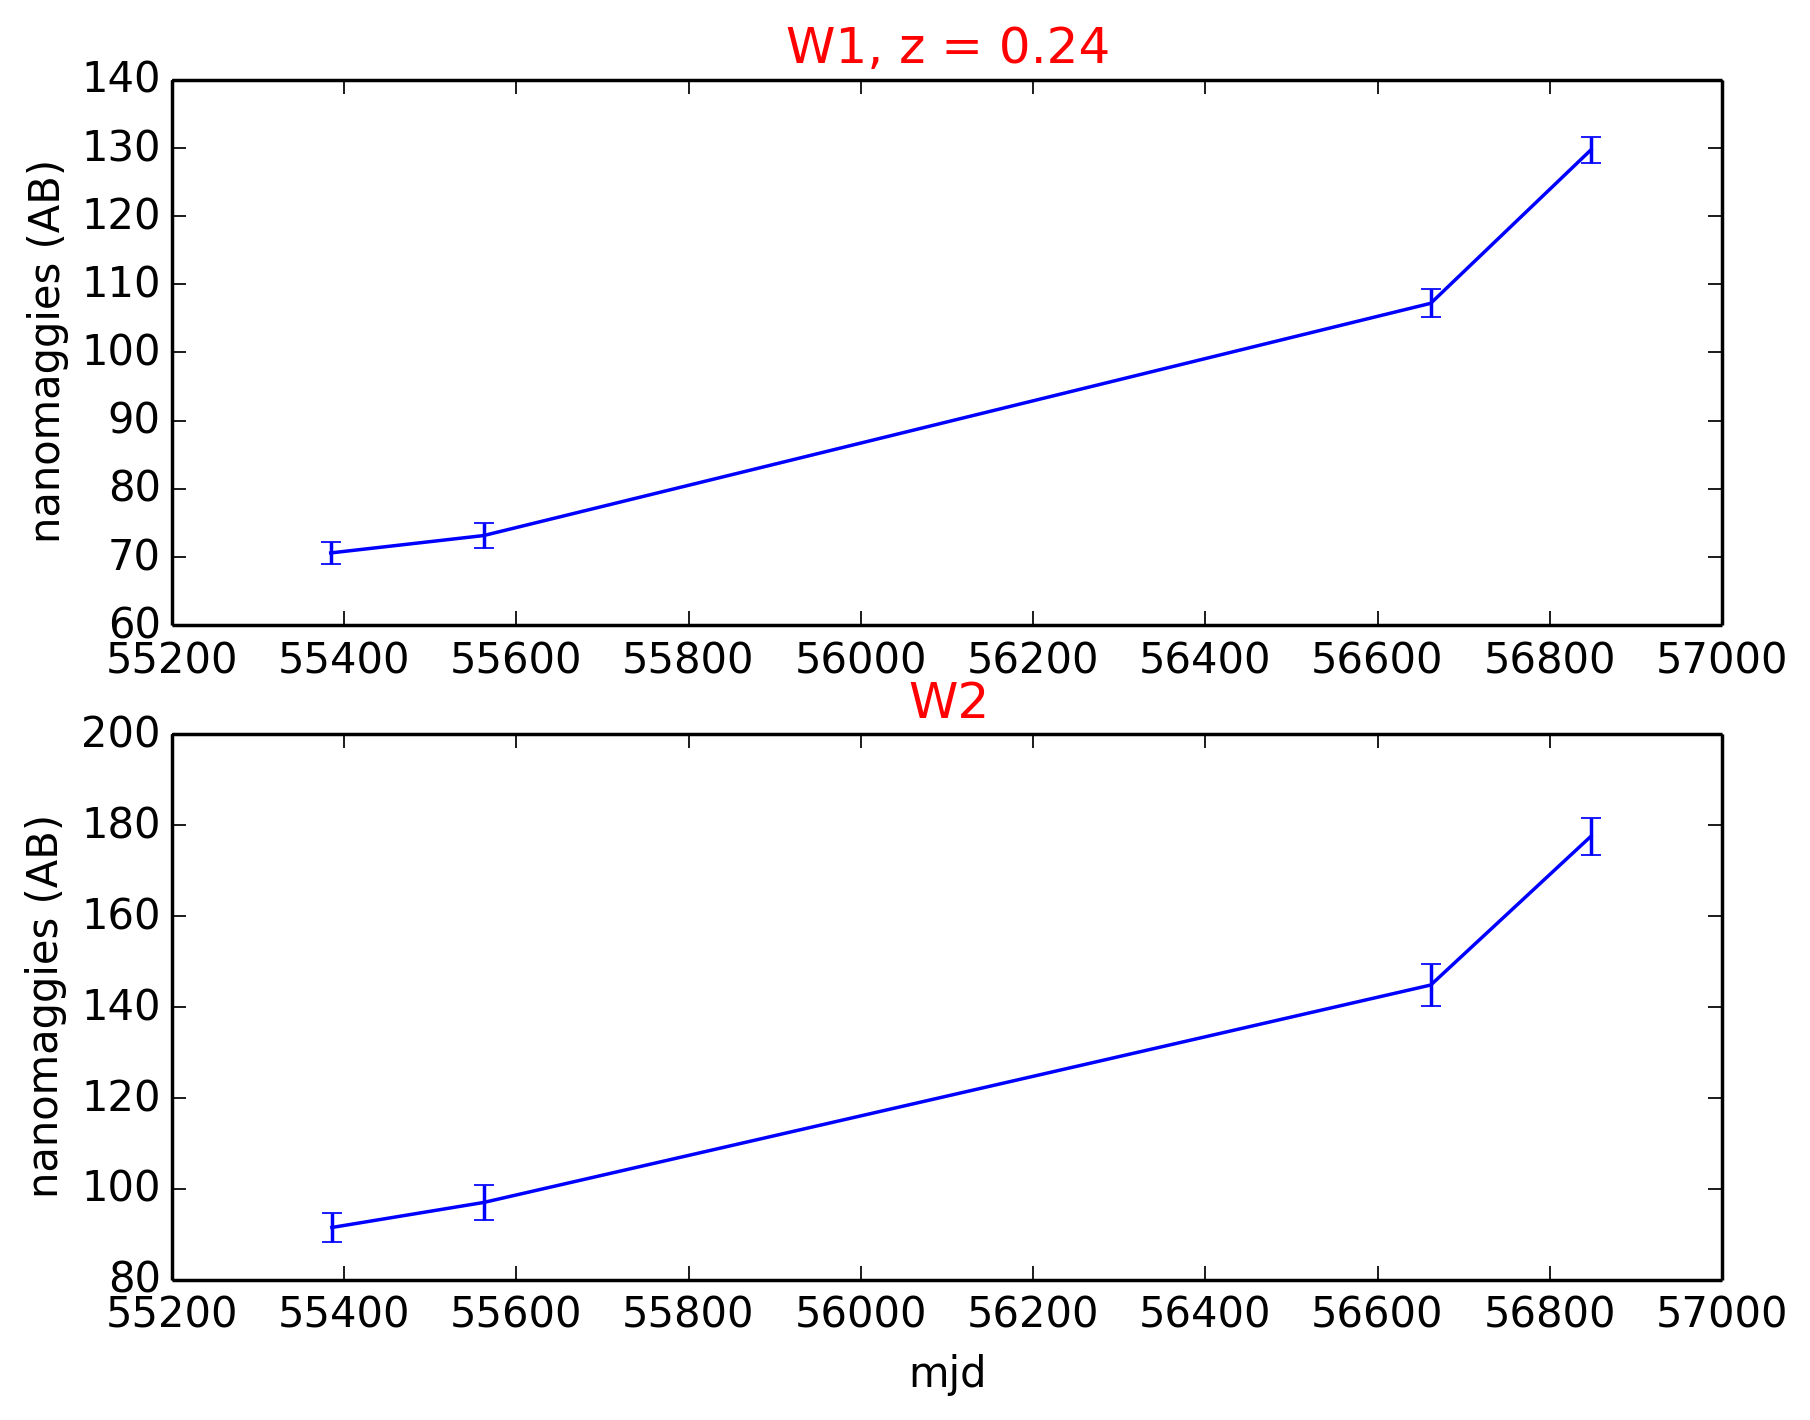
\includegraphics[width=8.00cm, height=6.50cm, 
    trim=0.0cm 0.0cm 0.0cm 0.0cm, clip]
    {lc_s003.png}
    \centering
    \caption[]{qso\_lightcurves\_0.5\_1.0/lc\_s003.png}
    \label{fig:lc_s003}
\end{figure}
  
\begin{figure*}
   %% trim=l b r t 
    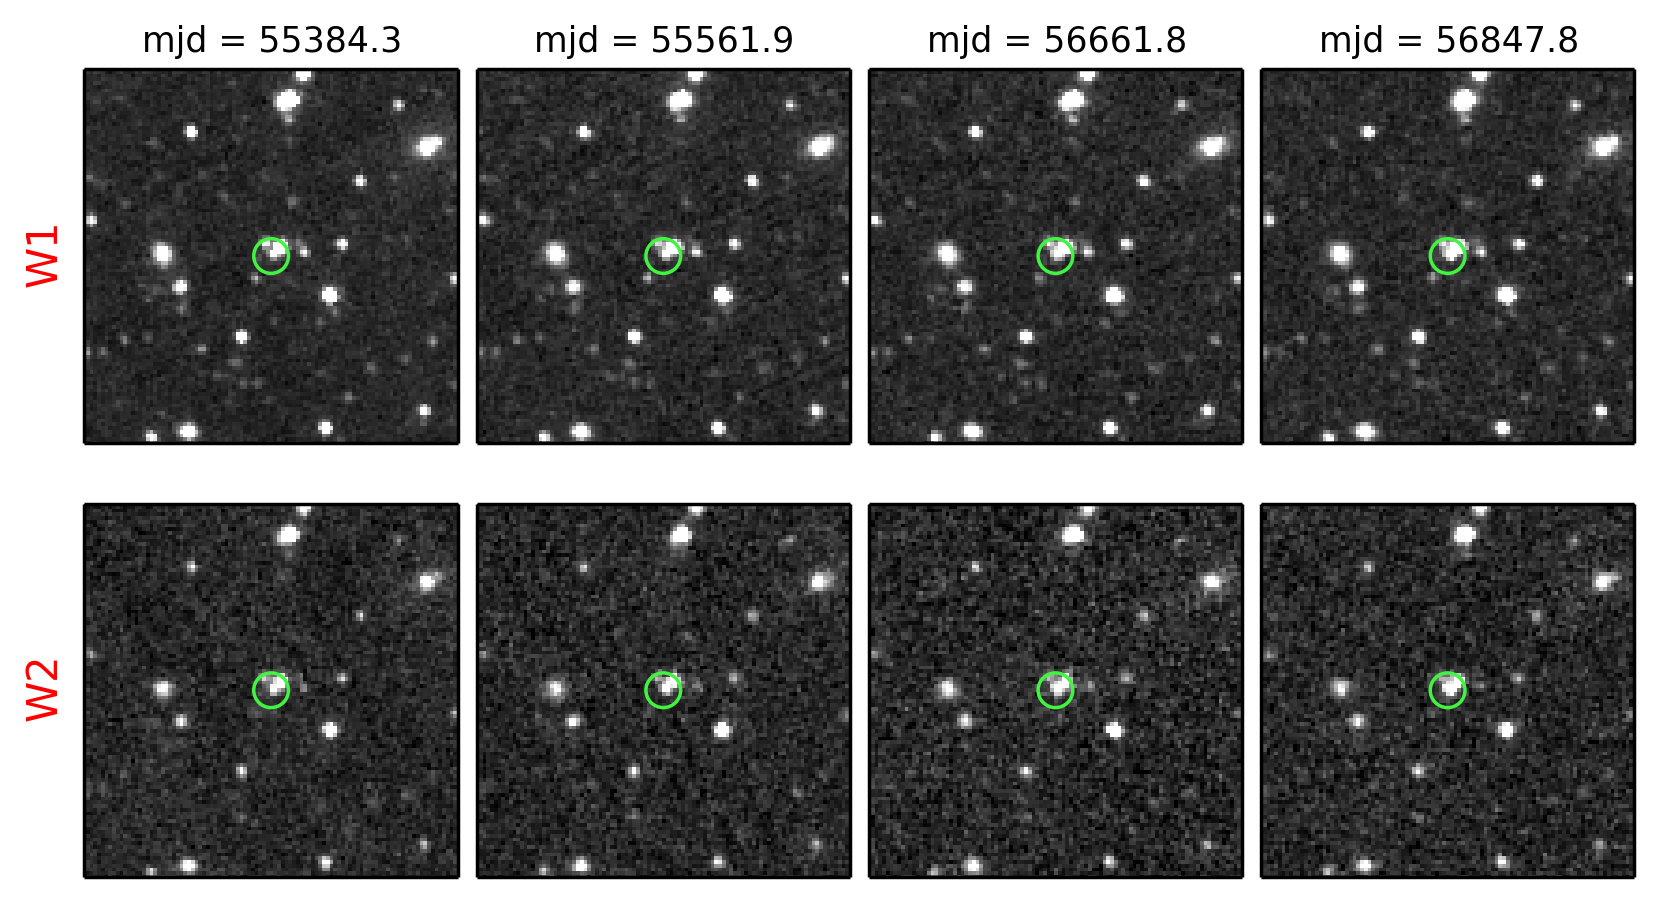
\includegraphics[width=14.00cm, height=7.50cm, 
    trim=0.0cm 0.0cm 0.0cm 0.0cm, clip] 
    {finder_s003.png}
    \centering
    % \vspace{-16pt}
    \caption[]{qso\_finders\_0.5\_1.0/finder\_s003.png}
    \label{fig:finder_s003}
\end{figure*}



%% 
%%  N. B. !!  N. B. !!   N. B. !!  N. B. !! 
%%  This is text from Aaron's email from 14th Dec, 2016
%%
%Hi Nic,
%
%I've made some WISE light curve catalogs in attempt to address your requests:

%% http://portal.nersc.gov/project/cosmo/temp/ameisner/dr3_wise_lc_sample.fits.gz
%% http://portal.nersc.gov/project/cosmo/temp/ameisner/dr3_wise_lc_metrics_all_qso.fits.gz
%


%The first has 248 rows, which are my preferred highly IR-variable
%sample of objects. The second is all 200,622 quasars that have "good"
%WISE light curves available in DR3.
%
%In each file, there are 3 extensions:
%
%ex = 0 -- my light curve summary metrics
%ex = 1 -- DECaLS DR3 Tractor data for each object (including WISE light curves)
%ex = 2 -- SDSS data for each object
%
%Let me know what you think. Hopefully tonight I'll be able to finish
%creating an updated set of finder charts, but we'll see how far I
%actually get on that...Thanks.
%
%-Aaron

A link to the key properties of our sample can be
\href{http://portal.nersc.gov/project/cosmo/temp/ameisner/qso\_pages\_v01/}
{\tt found here}.

%% 
%%  N. B. !!  N. B. !!   N. B. !!  N. B. !! 
%%  This is text from Aaron's email from 15th Feb, 2017, sent to Daniel, 
%%  for the WISE J1052+1519 outline/paper
%%
W1 and W2 lightcurves for $\sim$200,000 SDSS spectroscopic quasars were 
extracted from Data Release 3 (DR3) of the Dark Energy Camera Legacy Survey 
(DECaLS). These light curves span from the beginning of the WISE mission 
(2010 January) through the first-year of NEOWISER operations 
(2014 December). In detail, the W1/W2 light curves are obtained by performing 
forced photometry at the locations of DECam-detected optical sources. This 
forced photometry is performed on time-resolved unWISE coadds, each of which 
represents a stack with depth of coverage $\sim$12 exposures. A given sky 
location is observed by 
WISE for $\sim$1 day once every six months, which means that our forced 
photometry 
light curves typically have four coadd epochs available. Coadd epochs of a
given object are separated by a minimum of six months and a maximum of
four years. Our coaddition removes the possibility of probing variability on 
$\lesssim$1 day time scales, but it allows us to push $\sim$1.4 magnitudes 
deeper than individual exposures while removing virtually all single-exposure 
artifacts (e.g. cosmic rays and satellites).

$\sim$30,000 of the SDSS quasars with such W1/W2 lightcurves available are 
``IR-bright'', in the sense that they are above both the W1 and W2 single 
exposure thresholds and therefore detected at very high significance in our 
coadds. For this ensemble of objects, the typical variation in each quasar's 
measured (W1-W2) color is 0.06 magnitudes, which includes 
statistical and systematic errors expected to contribute variations
at the few hundredths of a mag level. The typical measured single-band scatter 
is 0.07 magnitudes in each of W1 and W2. A full characterization of
the typical mid-IR quasar variability will be presented separately 
(Ross et al., in preparation).

We undertook a search for extreme outliers relative to these trends. 
Specifically, we selected objects with the following characterisitcs.

% itemize type stuff
\begin{itemize}
\item Monotonic variation in both W1 and W2.
\item W1 versus W2 \textit{flux} correlation coefficient $>$0.9.
\item $>0.5$ mag peak-to-peak variation in either W1 or W2.
\end{itemize}


This yielded a sample of 248 sources. 31 of these are assumed to be blazars 
due to the presence of FIRST radio counterparts. Another 22 are outside of the 
FIRST  footprint, leaving 195 quasars in our IR-variable sample. We randomly 
selected five of these objects for follow-up spectroscopy with Palomar DBSP on
the night of 30 January 2017. WISE J1052+1519, one of these five, 
faded by 0.75 (0.9) mags in W1 (W2), and thus became 0.15 mags bluer in 
(W1-W2), making it a significant outlier in both single-band and IR color 
variability.



%%%%%%%%%%%%%%%%%%%%%%%%%%%%%%%%%%%%%%%%%%%%%%%%%%%%%%%%%%%%%%
%%%%%%%%%%%%%%%%%%%%%%%%%%%%%%%%%%%%%%%%%%%%%%%%%%%%%%%%%%%%%%
%%
%%     S E C T I O N     3      S E C T I O N     3       S E C T I O N     3       S E C T I O N     3  
%%     S E C T I O N     3      S E C T I O N     3       S E C T I O N     3       S E C T I O N     3  
%%     S E C T I O N     3      S E C T I O N     3       S E C T I O N     3       S E C T I O N     3  
%%
%%%%%%%%%%%%%%%%%%%%%%%%%%%%%%%%%%%%%%%%%%%%%%%%%%%%%%%%%%%%%%
%%%%%%%%%%%%%%%%%%%%%%%%%%%%%%%%%%%%%%%%%%%%%%%%%%%%%%%%%%%%%%
\section{Results}
Figures~\ref{fig:lc_s003} and \ref{fig:finder_s003} shows what the 
typical NEOWISER data look like for a non-typical quasar.
%%
Lorem ipsum dolor sit amet, consectetur adipiscing elit. Aliquam porta
sodales est, vel cursus risus porta non. Vivamus vel pretium
velit. Sed fringilla suscipit felis, nec iaculis lacus convallis
ac. Fusce pellentesque condimentum dolor, quis vehicula tortor
hendrerit sed. Class aptent taciti sociosqu ad litora torquent per
conubia nostra, per inceptos himenaeos. Etiam interdum tristique diam
eu blandit. Donec in lacinia libero.

    \begin{figure*}
      %% trim=l b r t 
      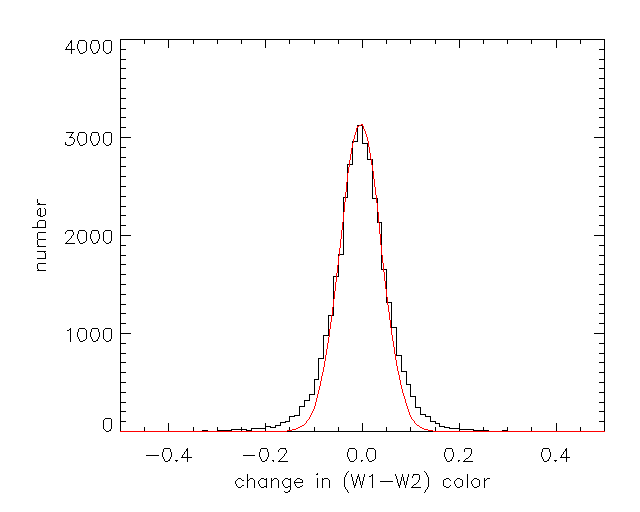
\includegraphics[width=7.50cm, height=7.50cm, 
      trim=0.0cm 0.0cm 0.0cm 0.0cm, clip]
      {w1w2_color_variation.png}
      \centering
      % \vspace{-16pt}
      \caption[]{The the variations in $(W1-W2)$ color using
        $\sim$37,500 data points from $\sim$9000 bright quasars.
        Overplotted is a Gaussian distribution, centered at -3.8 mmag 
        and with standard deviation of 0.06 mags (with a fit-by-eye ;-).}
      \label{fig:w1w2_color_variation}
    \end{figure*}
    \subsection{Color Changes}
    From Aaron's email:
    Figure~\ref{fig:w1w2_color_variation} shows the variations in the
    $(W1-W2)$ color, which is pretty narrow. Overplotted is a Gaussian
    distribution, centered at -3.8 mmag and with standard deviation of
    0.06 mags (with a fit-by-eye ;-)
    
    This histogram includes $\sim$37,500 data points from $\sim$9000
    bright quasars, that is, brighter than single-exposure detection limit in both
    W1 and W2. 
    % Let me know what you think. I can also try splitting by FIRST versus no FIRST.

    {\it NPR: It'd be friggin *awesome* if we could actually show a
      W1W2W3 RGB image of a quasar changing color!!!}

    \begin{figure*}
      %% trim=l b r t 
      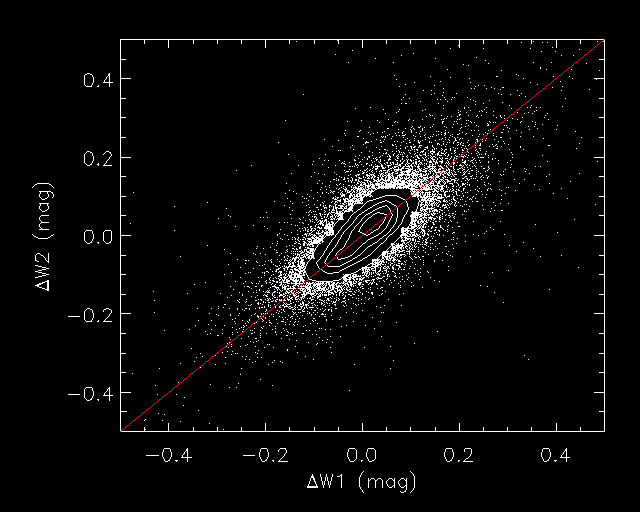
\includegraphics[width=7.50cm, height=7.50cm, 
      trim=0.0cm 0.0cm 0.0cm 0.0cm, clip]
      {scatter_dW1_dW2.png}
      \centering
      % \vspace{-16pt}
      \caption[]{The the variations in $(W1-W2)$ color using
        $\sim$37,500 data points from $\sim$9000 bright quasars. Overplotted
        is a Gaussian distribution, centered at -3.8 mmag and with standard
        deviation of 0.06 mags (with a fit-by-eye ;-).}
      \label{fig:scatter_dW1_dW2}
    \end{figure*}
    Figure~\ref{fig:scatter_dW1_dW2} has the same data as
    Fig~\ref{fig:w1w2_color_variation}, now in a scatterplot of
    $\Delta(W1)$ versus $\Delta(W2$). There is clearly some variation, and
    it is well-correlated between W1 and W2. The red line is $x=y$. 
    (I would guess this is real variation, but I'm still a little bit scared that
    you could have e.g. correlated background level issues in the coadds
    that imprint onto the fluxes.)

    \subsection{Extreme IR Variable Quasars vs. the general Quasar population}
    Turpis tincidunt quam consectetur non suscipit tellus placerat. Etiam
    sit amet justo condimentum sem scelerisque pharetra. Nullam sit amet
    neque eget quam tempor consectetur vel vitae massa. Nunc porttitor,
    quam in tempor pharetra, leo libero eleifend mi, ac ornare nibh eros
    vel purus. Pellentesque lobortis enim metus.
    

%%%%%%%%%%%%%%%%%%%%%%%%%%%%%%%%%%%%%%%%%%%%%%%%%%%%%%%%%%%%%%
%%%%%%%%%%%%%%%%%%%%%%%%%%%%%%%%%%%%%%%%%%%%%%%%%%%%%%%%%%%%%%
%%
%%     S E C T I O N     4      S E C T I O N     4       S E C T I O N     4       S E C T I O N     4
%%     S E C T I O N     4      S E C T I O N     4       S E C T I O N     4       S E C T I O N     4  
%%     S E C T I O N     4      S E C T I O N     4       S E C T I O N     4       S E C T I O N     4  
%%
%%%%%%%%%%%%%%%%%%%%%%%%%%%%%%%%%%%%%%%%%%%%%%%%%%%%%%%%%%%%%%
%%%%%%%%%%%%%%%%%%%%%%%%%%%%%%%%%%%%%%%%%%%%%%%%%%%%%%%%%%%%%%
\section{SDSS J110057.71-005304.5}

\begin{figure}
  %% trim=l b r t 
  \includegraphics[width=8.00cm, height=7.50cm, trim=0.0cm 0.0cm 0.0cm 0.0cm, clip]
  {../plots/w1100m0052_sdss.jpg
-rw-r--r--@ 1 npr1  admin  218664 Mar  3 09:03 ../plots/w1100m0052_hbeta.jpg
-rw-r--r--@ 1 npr1  admin  214894 Mar  3 09:03 ../plots/w1100m0052_halpha.jpg
-rw-r--r--@ 1 npr1  admin  182067 Mar  3 09:03 ../plots/w1100m0052.jpgfig1.png}
  \centering
  % \vspace{-16pt}
  \caption[]{
    {\bf All from DJS's email:} The distribution of the maxima and
    minima flux in $W1$ for the $\sim$240k high-confidence quasars in the
    SDSS-III: BOSS DR12.  The red distribution is if one replaces fluxes
    with a mean flux$+$measurement error for each observation.  Note,
    since the log is being plotted, the difference between the two lines
    shows a significant variable population.  There are $\sim$1000 quasars
    where the $W1$ flux varies by more than a factor of 2 with a $>5$
    sigma confidence.  Some have a poor $\chi{^2}$ fits.
  }
 \label{fig:maxminflux}
\end{figure}

\subsection{General Observational Details}
SDSS J110057.71-005304.5, hereafter J110057, was discovered by 
the Sloan Digital Sky Survey in 2000. 
 J110057 was imaged in Run 756 (which makes up Stripe 10), 
and satisfied a number of spectroscopic targettings flags
(SERENDIP\_BLUE, ROSAT\_D,  ROSAT\_C,  ROSAT\_B, QSO\_SKIRT, ROSAT\_A)
making it a quasar target. A spectrum was obtain on MJD 51908, on Plate 
277, Fiber 212, and the spectrum of a $z=0.378\pm0.00003$ was

In the DECaLS, the 
DECaLS brick containing J110057.71-005304.5.

number of exposures in g : 8\\
number of exposures in r : 3\\
number of exposures in z : 9 \\

$56707.146 <= g_MJD <= 56727.201$
$56367.091 <= r_MJD <= 56367.230$
$56383.159 <= z_MJD <= 57398.350$

As can be seen, the $g-$ and $r-$band observations have fairly limited
time spans, and are separated by roughly a year. The $z$-band observations
span almost 3 years.  The DESI imaging brick name is 1651m010. 
%%  I've attached the CCDs file, which comes from:
%%  /project/projectdirs/cosmo/data/legacysurvey/dr3.1/coadd/165/1651m010/legacysurvey-1651m010-ccds.fits
%%  -Aaron

Second epoch spectrum from BOSS. 

A third epoch spectrum was obtained from the Palomar 5m 
telescoep and 
 and 600s+300s on the second.  Conditions were good.

Attached are a bunch of plots, showing both the new data and
comparison of the new data to archival SDSS/BOSS data.  Take-aways:

- W1052+1519 data is much better than the data we got in late January
in 2-4 arcsec seeing.  We should consider this as superseding those
data, but still telling the same story.

- W1100-0052 is a bit more confounding.  The continuum straddling MgII
is now blue, as it was for the SDSS spectrum in 2000, as opposed to
red, as it was for the BOSS spectrum in 2010.  I'm cautiously
optimistic that the strange BOSS continuum shape is real rather than
instrumental, but it's still nagging at me that it might not be real.

- W1100-0052 SDSS spectrum has an interesting contiuum chunk missing
at ~4300 A, which largely fills in since then??!!!   A month ago we
would have jumped up and down claiming a gap in the accretion disk
caused by an SMBH binary, but newer calculations suggest such a gap is
a much wider, shallower deviation.

- bluest P200 continuum (<3800 A) for W1100-0552 has an instrumental
fringing issue which causes the high frequency gunkiness, to use the
technical term.  This is a known issue with the DBSP
instrument/detector.
Lorem ipsum dolor sit amet, consectetur adipiscing elit. Aliquam porta
sodales est, vel cursus risus porta non. Vivamus vel pretium
velit. Sed fringilla suscipit felis, nec iaculis lacus convallis
ac. Fusce pellentesque condimentum dolor, quis vehicula tortor
hendrerit sed. Class aptent taciti sociosqu ad litora torquent per
conubia nostra, per inceptos himenaeos. Etiam interdum tristique diam
eu blandit. Donec in lacinia libero.

Sed elit massa, eleifend non sodales a, commodo ut felis. Sed id
pretium felis. Vestibulum et turpis vitae quam aliquam convallis. Sed
id ligula eu nulla ultrices tempus. Phasellus mattis erat quis metus
dignissim malesuada. Nulla tincidunt quam volutpat nibh facilisis
euismod. Cras vel auctor neque. Nam quis diam risus.

Nunc semper quam et leo interdum vulputate eu quis magna. Sed nec arcu
at orci egestas convallis. Aenean quam velit, aliquam vitae viverra
in, elementum vel elit. Nunc suscipit aliquet sapien a suscipit. Cras
nulla ipsum, posuere eu fringilla sit amet, dapibus ultricies
nulla. Nullam eu augue id purus mollis dignissim sed et
libero. Phasellus eget justo sed neque pellentesque egestas nec id
arcu. Donec facilisis pulvinar sapien et fringilla. Suspendisse
vestibulum rhoncus sapien id laoreet. Morbi et orci vitae tortor
imperdiet imperdiet. In hac habitasse platea dictumst. Vivamus vel
neque id mi ultrices tristique. Integer quam libero, ornare vel
gravida in, feugiat a ante. Nam dapibus, tellus vitae pellentesque
cursus, dui nisl egestas augue, non fermentum nisl est nec
nisi. Vestibulum nec mi justo, eget dapibus velit.

Cras in laoreet mauris. Vivamus nec nulla a dui commodo
adipiscing. Proin vulputate lectus nec arcu iaculis sit amet auctor
ligula ultricies. Phasellus condimentum gravida tincidunt. Phasellus
et mauris ac nibh vestibulum vehicula. Morbi et augue id purus gravida
sagittis quis in sem. Phasellus quis risus bibendum eros luctus
auctor.

Etiam mollis viverra nisi eget aliquet. Aliquam erat volutpat. Vivamus
tristique, nisl eu malesuada semper, libero tortor convallis elit, a
scelerisque orci nisi lacinia turpis. In lacinia ultrices
volutpat. Proin ultrices luctus tellus, in placerat eros tincidunt
id. Ut varius iaculis quam in consequat. Nulla nec orci est, sit amet
pellentesque nisl. Mauris non cursus lectus. Praesent placerat leo vel
erat gravida lacinia. Donec vehicula consectetur lectus vitae
luctus. Praesent nisl justo, laoreet elementum facilisis vel,
tristique ac enim. Etiam vel quam ut quam eleifend
tincidunt. Suspendisse sit amet eros vel elit ullamcorper
laoreet. Etiam venenatis sodales turpis, nec lacinia ligula hendrerit
nec. Nam eu vulputate purus. Quisque facilisis congue metus, sed
imperdiet lorem rhoncus sit amet.

Proin non tempus velit. Etiam laoreet, enim nec scelerisque dictum,
tortor massa tempor enim, id pretium justo quam ac lectus. Maecenas
diam nibh, interdum at lobortis sit amet, dignissim et quam. Sed
tincidunt faucibus risus, congue tempus nisl consectetur
eget. Suspendisse venenatis turpis ut risus aliquam interdum. In at
velit sed ligula dictum dignissim ut et dui. Curabitur ac scelerisque
purus.



%%%%%%%%%%%%%%%%%%%%%%%%%%%%%%%%%%%%%%%%%%%%%%%%%%%%%%%%%%%%%%
%%%%%%%%%%%%%%%%%%%%%%%%%%%%%%%%%%%%%%%%%%%%%%%%%%%%%%%%%%%%%%
%%
%%     S E C T I O N     5      S E C T I O N     5       S E C T I O N     5       S E C T I O N     5
%%     S E C T I O N     5      S E C T I O N     5       S E C T I O N     5       S E C T I O N     5  
%%     S E C T I O N     5      S E C T I O N     5       S E C T I O N     5       S E C T I O N     5  
%%
%%%%%%%%%%%%%%%%%%%%%%%%%%%%%%%%%%%%%%%%%%%%%%%%%%%%%%%%%%%%%%
%%%%%%%%%%%%%%%%%%%%%%%%%%%%%%%%%%%%%%%%%%%%%%%%%%%%%%%%%%%%%%
\section{Discussion and Conclusions}
Sed non felis iaculis dui iaculis mattis facilisis ullamcorper
ipsum. Donec erat nunc, consectetur et ornare in, egestas vitae
mauris. Praesent suscipit rutrum purus, in interdum tellus euismod sit
amet. Nulla facilisi. Etiam nisl ligula, vehicula at fringilla et,
sagittis eu odio.

Our conclusions are thus: 
\begin{itemize}
    \item{Hendrerit pretium commodo. Cras dapibus fringilla dolor a
        ultrices. Morbi bibendum neque in magna pellentesque rhoncus. Sed
        vitae lorem lacus.}
    \item{Pellentesque nec justo et dolor scelerisque
        fermentum. Vivamus augue libero, fermentum id tristique at, suscipit
        ultricies turpi.}
    \item{Cras in laoreet mauris. Vivamus nec nulla a dui commodo
        adipiscing. Proin vulputate lectus nec arcu iaculis sit amet auctor
        ligula ultricies. Phasellus condimentum gravida tincidunt. Phasellus
        et mauris ac nibh vestibulum vehicula.}
\end{itemize}

Morbi et augue id purus gravida sagittis quis in sem. Phasellus quis
risus bibendum eros luctus auctor. Proin non tempus velit. Etiam
laoreet, enim nec scelerisque dictum, tortor massa tempor enim, id
pretium justo quam ac lectus. Maecenas diam nibh, interdum at lobortis
sit amet, dignissim et quam. Sed tincidunt faucibus risus, congue
tempus nisl consectetur eget. Suspendisse venenatis turpis ut risus
aliquam interdum. In at velit sed ligula dictum dignissim ut et
dui. Curabitur ac scelerisque purus.



\section{Acknowledgments}
We thank the IPAC team for the Explanatory Supplement to the WISE
All-Sky and AllWISE Data Release Products resource.  NEOWISE and
NEOWISE-R makes use of data from WISE, which is a joint project of the
University of California, Los Angeles, and the Jet Propulsion
Laboratory/California Institute of Technology, and NEOWISE, which is a
project of the Jet Propulsion Laboratory/California Institute of
Technology. WISE and NEOWISE are funded by the National Aeronautics
and Space Administration.

This research made use of the NASA Astrophysics Data System.  This
research also made use of the \href{www.astropy.org}{\tt astropy.org}
codebase (proper citation).  The data and code used herein will become
publicly available at \href{\tt
http://www.legacysurvey.org/dr3/Extreme_wise_quasars/} upon
publication of the paper.

N.P.R. acknowledges support from the STFC and the Ernest Rutherford
Fellowship scheme.
%N.P.R. thanks Nathan Bourne for useful discussions on infrared-to-radio flux ratios. 

Funding for the SDSS and SDSS-II has been provided by the Alfred
P. Sloan Foundation, the Participating Institutions, the Na- tional
Science Foundation, the US Department of Energy, the National
Aeronautics and Space Administration, the Japanese Monbukagakusho, the
Max Planck Society, and the Higher Ed- ucation Funding Council for
England. The SDSS web site is
\href{http://www.sdss.org/}{http://www.sdss.org}.

Funding for SDSS-III has been provided by the Alfred P. Sloan
Foundation, the Participating Institutions, the National Science
Foundation, and the U.S. Department of Energy. The SDSS-III web site
is \href{http://www.sdss3.org/}{http://www.sdss3.org/}.  SDSS-III is
managed by the Astrophysical Research Consortium for the Participating
Institutions of the SDSS-III Collaboration including the University of
Arizona, the Brazilian Participation Group, Brookhaven National
Laboratory, University of Cambridge, University of Florida, the French
Participation Group, the German Participation Group, the Instituto de
Astrofisica de Canarias, the Michigan State/Notre Dame/JINA
Participation Group, Johns Hopkins University, Lawrence Berkeley
National Laboratory, Max Planck Institute for Astrophysics, New Mexico
State University, New York University, Ohio State University,
Pennsylvania State University, University of Portsmouth, Princeton
University, the Spanish Participation Group, University of Tokyo,
University of Utah, Vanderbilt University, University of Virginia,
University of Washington, and Yale University.  \\ {\it Facilities:
SDSS, BOSS, WISE, CTIO Blanco+DECam}




\appendix
\section{Technical Details}
All good papers have to have an Appendix. 


\bibliographystyle{mn2e} 
\bibliography{tester_mnras}




\end{document}
